\chapter{Despliegue} \label{sec:deployment}
    En esta sección se abordan aspectos relevantes en relación con el despliegue de la aplicación web desarrollada. 
    
    \section{Heroku} \label{sec:heroku}
    Desde el surgimiento de las tecnologías web hasta nuestros días, las herramientas a disposición de los desarrolladores para abrir al público una aplicación web se han incrementado considerablemente. Desde tener cada uno que adquirir, configurar y mantener el hardware necesario, a los modernos servicios de \emph{cloud-computing}.
    
    La presente aplicación web ha sido desplegada en Heroku, una infraestructura de \emph{cloud-computing} que sigue el modelo \emph{platform as a service}.
    
    Aparte de las ventajas que de por sí ofrece el modelo de computación en la nube, Heroku destaca por proporcionar una experiencia de desarrollo excepcional. Así, los desarrolladores sólo tienen que enfocarse en las tareas propias de programación, reduciéndose las labores de despliegue a unas pocas configuraciones y a efectuar un \emph{git push}. Literalmente, tras una mínima configuración (en el común de los casos sólo necesaria la primera vez), desplegar la aplicación en Heroku se realiza enviando el repositorio Git a la plataforma (existen otras formas, como integrar GitHub o IntelliJ IDEA con Heroku). Es decir, a Heroku se le envía el código fuente del proyecto, tras lo cual automáticamente lo construye, configura el hardware necesario, y lo despliega.
    
    Las aplicaciones desplegadas en Heroku son ejecutadas en contenedores Linux, denominados en la jerga Heroku como \href{https://devcenter.heroku.com/articles/dynos}{\emph{dynos}}. Cada uno de estos contenedores puede tener una configuración \emph{Web} (los únicos que admiten tráfico HTTP), \emph{Worker} o \emph{One-off}. Además, Heroku ofrece varios tipos de \emph{dynos}, cada uno adaptado a diferentes necesidades, desde pequeños proyectos hasta servicios en producción de gran tráfico. Así, como se muestra en la figura \ref{fig:dyno_types}, tomada de la documentación oficial, cada tipo de dyno posee diferentes características, como la memoria disponible o la exclusividad de los recursos que utiliza.
    
    \begin{figure}[hbt!]
       	\centering
       	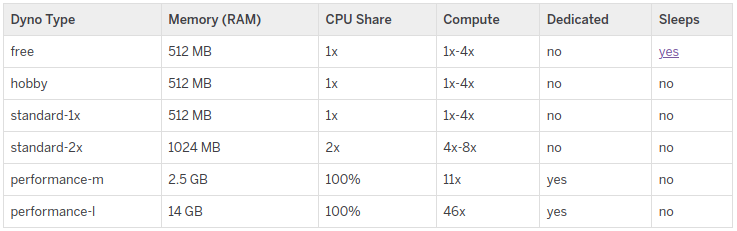
\includegraphics[width=0.9\textwidth,keepaspectratio]{dyno_types}
       	\caption{Diferentes tipos de \emph{dynos} en Heroku}
       	\label{fig:dyno_types}
    \end{figure}
    
    FirstMarket ha sido desplegada en Heroku usando un \emph{dyno} del tipo \emph{hobby} con configuración \emph{web}. En la figura \ref{fig:heroku} se muestra el panel central desde donde se gestiona el despliegue.
    
    \begin{figure}[hbt!]
       	\centering
       	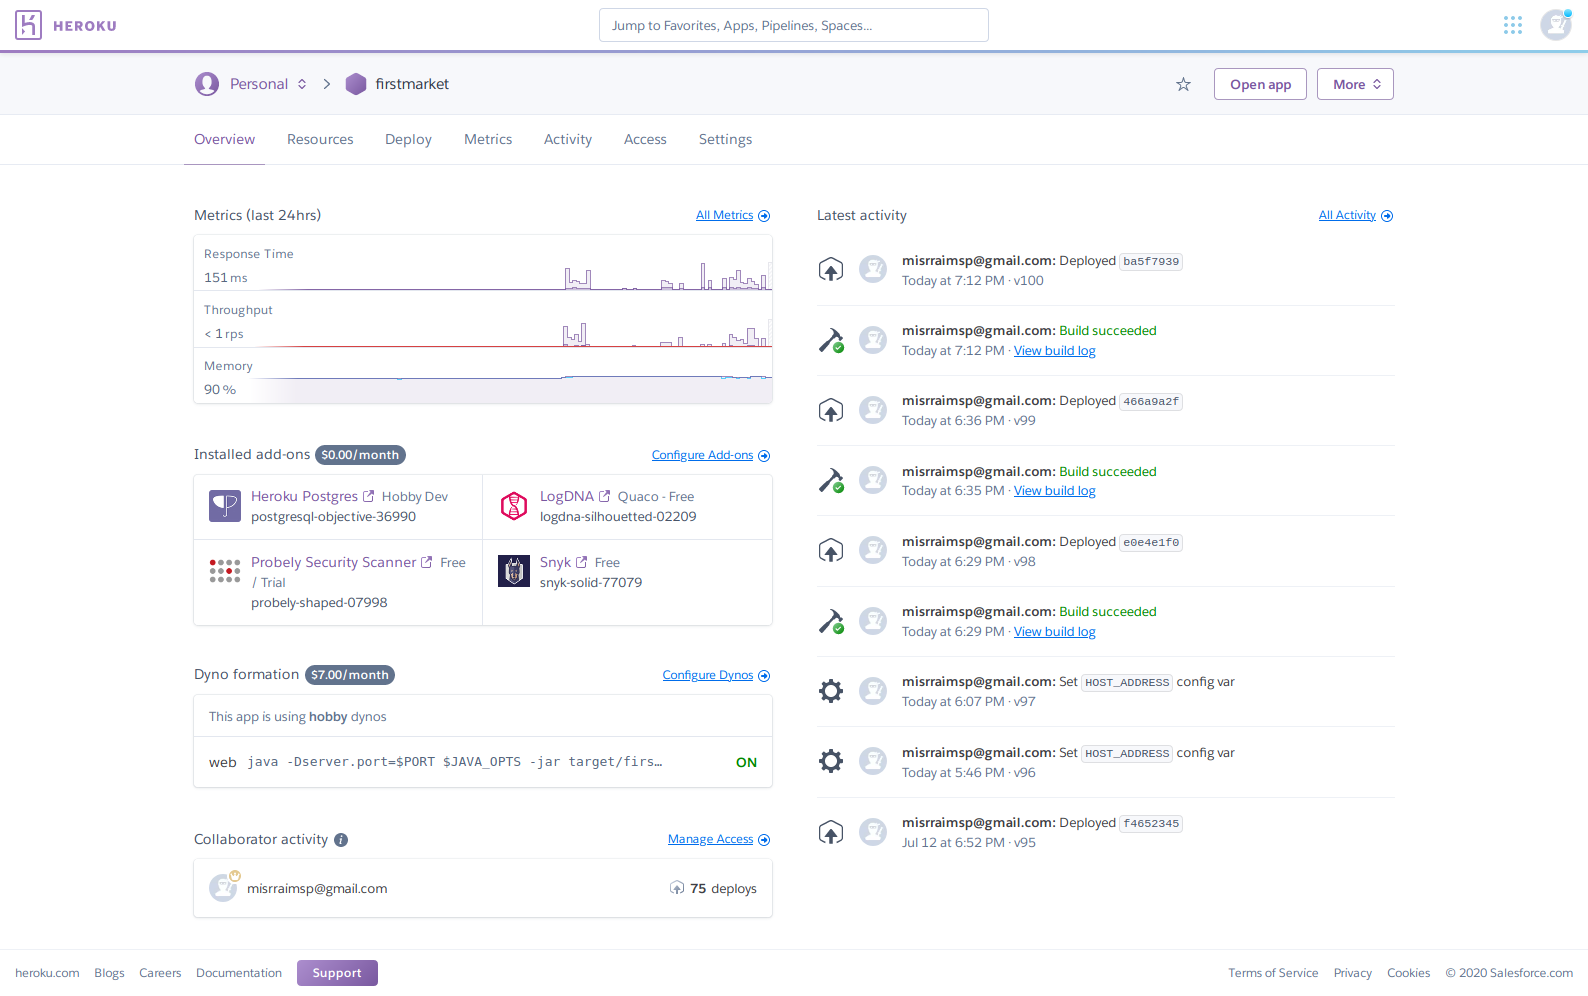
\includegraphics[width=\textwidth,keepaspectratio]{heroku}
       	\caption{Panel de control del despliegue de FirstMarket en Heroku}
       	\label{fig:heroku}
    \end{figure}

    \section{Heroku Add-ons} \label{sec:addons}
    Un aspecto interesante de Heroku es su oferta de \emph{Add-ons}, accesible en su \href{https://elements.heroku.com/addons}{marketplace}. Se trata de módulos que se pueden añadir a la aplicación web, algunos gratuitos y otros de pago. La aplicación web desarrollada hace uso de los siguientes:
    
    \begin{itemize}
       	\item[-] \href{https://elements.heroku.com/addons/heroku-postgresql}{Heroku Postgres}. Este es el servicio de base de datos utilizado para la capa de persistencia de la aplicación web cuando está desplegada en Heroku. El plan contratado es el gratuito, estando restringido a que el total de filas en la base de datos no supere las 10000, y con un máximo de 20 conexiones disponibles. En la figura \ref{fig:herokupostgres} se muestra el panel central de este servicio. Destacar la posibilidad de crear \emph{Dataclips}, que son consultas almacenadas sobre la base de datos. Como se aprecia, el número de filas se encuentra por debajo del límite.
       	
       	\begin{figure}[hbt!]
       		\centering
       		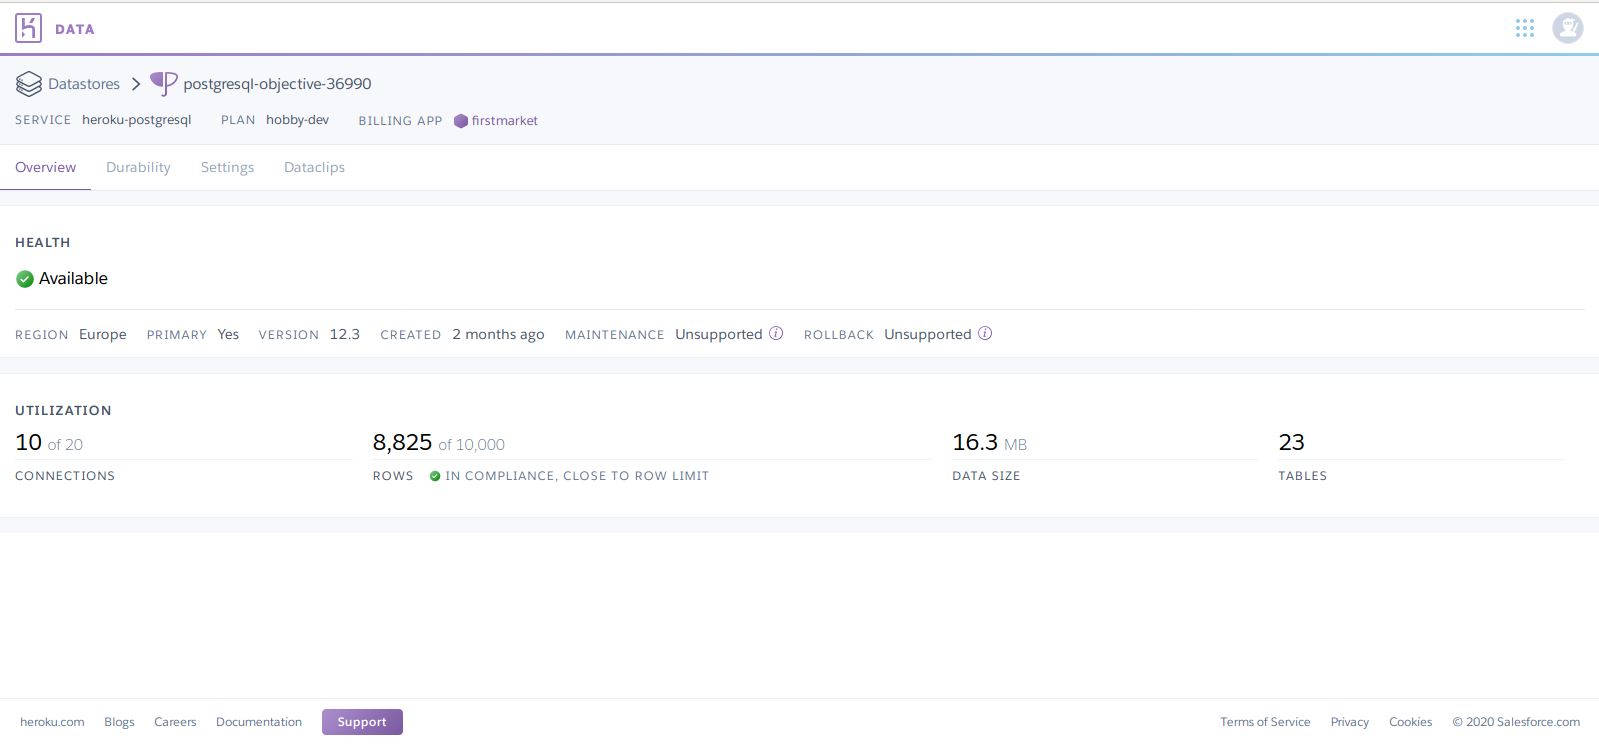
\includegraphics[width=\textwidth,keepaspectratio]{herokupostgres}
       		\caption{Panel de control de Heroku Postgres}
       		\label{fig:herokupostgres}
       	\end{figure}
       	
       	\item[-] \href{https://elements.heroku.com/addons/logdna}{LogDNA}. Este servicio permite acceder a los registros emitidos, tanto por la Heroku como por la aplicación web, de una manera sencilla a través del navegador. Tiene multitud de opciones de configuración, siendo la interfaz gráfica la mostrada en la figura \ref{fig:logdna}.
       	
       	\begin{figure}[hbt!]
       		\centering
       		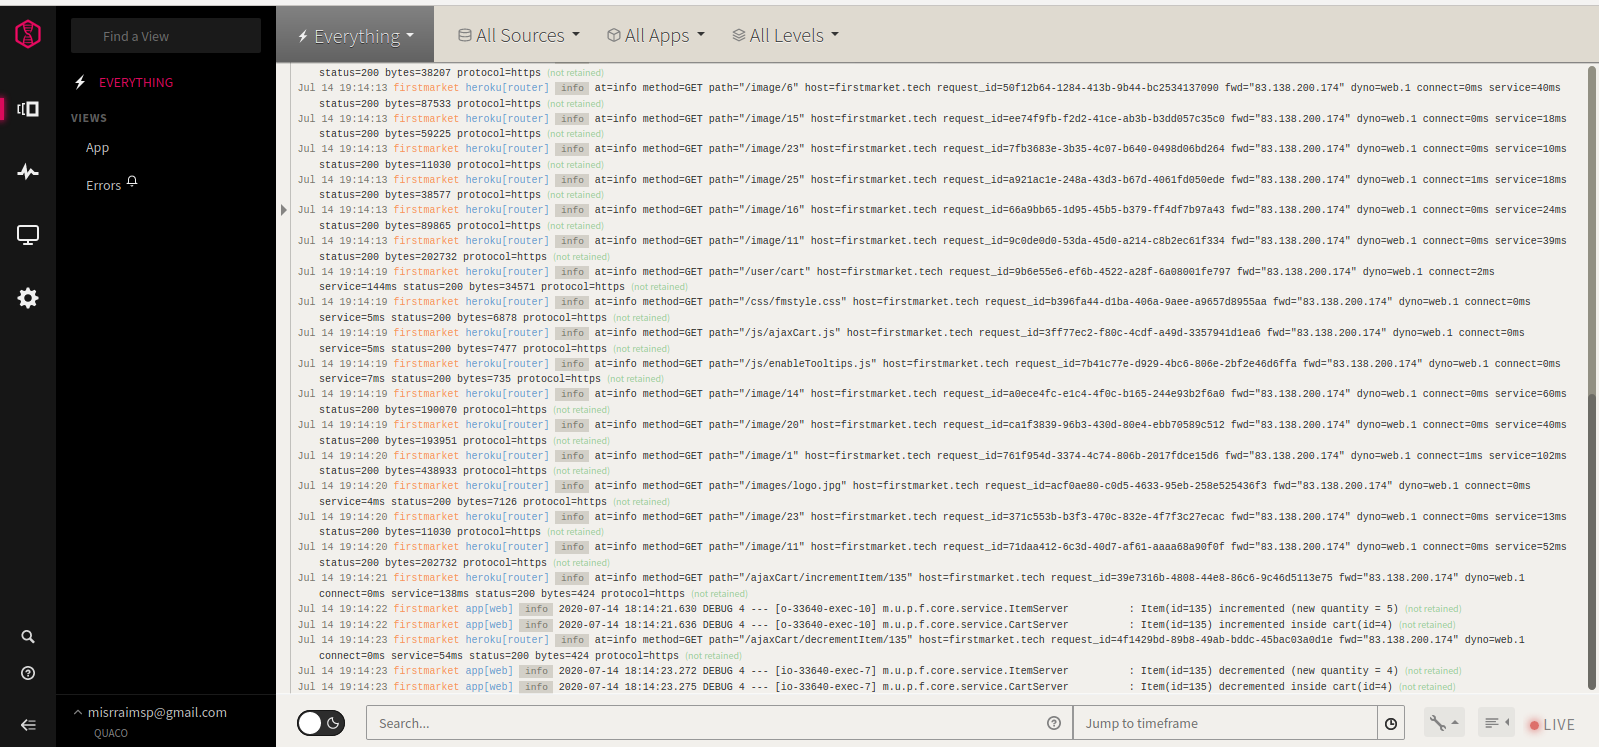
\includegraphics[width=\textwidth,keepaspectratio]{logdna}
       		\caption{Registros con LogDNA}
       		\label{fig:logdna}
       	\end{figure}
       	
       	\item[-] \href{https://elements.heroku.com/addons/probely}{Probely}. Este es un servicio de detección de vulnerabilidades de seguridad. En su versión pro, a la cual se ha tenido acceso gratuito durante dos semanas, permite realizar multitud de pruebas a la aplicación web, generando un informe de forma automática con los problemas encontrados y sus posibles soluciones. Se evaluó la aplicación web desarrollada con dos test diferentes: un análisis en profundidad estándar de Probely y un análisis OWASP top 10. Los resultados son comentados en la sección \ref{sec:vulnerabilities}.
       	\item[-] \href{https://elements.heroku.com/addons/snyk}{Snyk}. Este add-on revisa las dependencias del proyecto en busca de vulnerabilidades de seguridad conocidas. En su versión gratuita permite realizar hasta 200 test al mes, pero no emite informes es formato pdf. Los resultados son comentados en la sección \ref{sec:vulnerabilities}.
    \end{itemize}

	\section{firstmarket.tech}
	Por defecto, Heroku muestra sus aplicaciones web en el dominio \emph{nombre\_aplicacion.herokuapp.com}, aunque permite de forma sencilla y sin coste adicional \href{https://devcenter.heroku.com/articles/custom-domains}{añadir otros dominios}. Así, para la apertura al público de FirstMarket se ha comprado el dominio \textbf{\emph{firstmarket.tech}}, a través del registrador de dominios \href{https://www.namecheap.com/}{namecheap}.
	
	Una vez adquirido el dominio, se debe configurar sus registros DNS para que apunten a Heroku, que es donde se está ejecutando la aplicación. La figura \ref{fig:dns} muestra dichos registros DNS configurados en el panel de control que ofrece namecheap.
	
	\begin{figure}[hbt!]
		\centering
		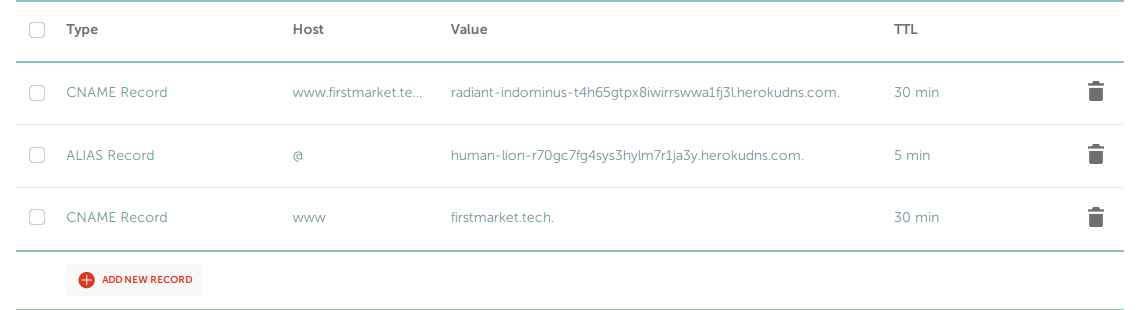
\includegraphics[width=\textwidth,keepaspectratio]{dns}
		\caption{Configuración de los registros DNS de firstmarket.tech en namecheap}
		\label{fig:dns}
	\end{figure}